\documentclass[a5paper]{article}
\usepackage[a5paper, top=8mm, bottom=8mm, left=8mm, right=8mm]{geometry}

\usepackage{polyglossia}
\setdefaultlanguage[babelshorthands=true]{russian}

\usepackage{fontspec}
\setmainfont{FreeSerif}
\newfontfamily{\russianfonttt}[Scale=0.7]{DejaVuSansMono}

\usepackage[font=scriptsize]{caption}

\usepackage{amsmath}
\usepackage{amssymb,amsfonts,textcomp}
\usepackage{color}
\usepackage{array}
\usepackage{hhline}
\usepackage{cite}
\usepackage{textcomp}

\usepackage[hang,multiple]{footmisc}
\renewcommand{\footnotelayout}{\raggedright}

\PassOptionsToPackage{hyphens}{url}\usepackage[xetex,linktocpage=true,plainpages=false,pdfpagelabels=false]{hyperref}
\hypersetup{colorlinks=true, linkcolor=blue, citecolor=blue, filecolor=blue, urlcolor=blue, pdftitle=1, pdfauthor=, pdfsubject=, pdfkeywords=}

\newlength\Colsep
\setlength\Colsep{10pt}

\usepackage{tabu}

\usepackage{graphicx}
\usepackage{indentfirst}
\usepackage{multirow}
\usepackage{subfig}
\usepackage{footnote}
\usepackage{minted}

\newcommand{\todo}[1] {
\begin{center}\textcolor{red}{TODO: #1}\end{center}
}

\sloppy
\pagestyle{plain}

\title{Лекция 1: Об архитектуре}
\author{Юрий Литвинов\\\small{yurii.litvinov@gmail.com}}

\begin{document}

\maketitle
\thispagestyle{empty}

\section{Введение}

% Источник: википедия (https://ru.wikipedia.org/wiki/%D0%90%D1%80%D1%85%D0%B8%D1%82%D0%B5%D0%BA%D1%82%D1%83%D1%80%D0%B0_%D0%BF%D1%80%D0%BE%D0%B3%D1%80%D0%B0%D0%BC%D0%BC%D0%BD%D0%BE%D0%B3%D0%BE_%D0%BE%D0%B1%D0%B5%D1%81%D0%BF%D0%B5%D1%87%D0%B5%D0%BD%D0%B8%D1%8F, https://en.wikipedia.org/wiki/Software_architecture), статья Perry, Dewayne E., and Alexander L. Wolf. "Foundations for the study of software architecture." ACM SIGSOFT Software engineering notes 17.4 (1992): 40-52., лекция Тимофея Брыксина (https://docs.google.com/document/d/1-yC3j5ZTgswMhXS7WI-1F4ZSWFXUhd2Dw3LvbfnGyL0/edit#heading=h.n859ee7jvlvk), глава 1 книги Z. Quin, J. Xing, X.Zheng, "Software Architecture",  Zhejiang University Press, 2008, 337pp.
В этом курсе речь пойдёт про архитектуру программного обеспечения. Первое, что нужно сделать --- это определиться, что именно мы называем архитектурой, и, собственно, этому и будет посвящена первая лекция. Тут оказывается, что не всё так просто, и все понимают под словом <<архитектура>> что-то своё. Формального определения понятия <<Архитектура ПО>> не существует. В академической среде под архитектурой понимают больше средства формального доказательства некоторых <<архитектурных>> свойств системы, исследуют формальные языки описания архитектуры и математические формализмы, с этим связанные (например, CSP\footnote{Communicating Sequential Processes}, $\pi$-исчисление). В индустриальной среде как правило даже не знают, что так можно, и понимают под архитектурой <<совокупность важнейших решений об организации программной системы>> (\textcopyright Википедия) --- декомпозицию системы на компоненты и способы взаимосвязи между компонентами. Так что мы начнём несколько издалека.

\section{Архитектура? Какая архитектура?}

\subsection{О программе и программном продукте}


\noindent\begin{minipage}{\textwidth}
	\begin{minipage}[c][6cm][c]{\dimexpr0.7\textwidth-0.5\Colsep\relax}
		Вообще, об архитектуре программного обеспечения заговорили только в начале 1990-х годов, что, конечно, уже прошлый век, но всё равно удивительно недавно --- люди как-то программировали компьютеры с 1940-х годов, а UNIX, Windows, C++, Pascal и т.д. появились тогда, когда архитектуры как отдельной области программной инженерии ещё по сути не существовало. Многие профессиональные разработчики до сих пор <<не верят>> в архитектуру, многим студентам тоже кажется, что программирование --- это больше про <<фигачить код>>, а архитектура --- это что-то ненужное, чем занимаются в огромных неповоротливых организациях. Разберёмся, почему.
	\end{minipage}\hfill
	\begin{minipage}[c][6cm][c]{\dimexpr0.3\textwidth-0.5\Colsep\relax}
		
\includegraphics[width=\textwidth]{whatArchitecture.png}
	\end{minipage}%
\end{minipage}

На рисунке~\ref{figure:brooksSquare} воспроизведена знаменитая иллюстрация из ещё более знаменитой книги Фредерика Брукса <<Мифический человеко-месяц, или Как создаются программные системы>>\footnote{Брукс Ф. Мифический человеко-месяц или как создаются программные системы. -- СПб : Символ-плюс, 2010, 304 с.}. В левом верхнем углу <<Программа>> --- это кусок кода, который запускается и делает то, что нужно, на машине разработчика и если входные данные корректны и ничего плохого не происходит (работает так называемая <<основная ветка>> программы). Иногда, потому что никто не удосужился хорошенько его протестировать или попытаться доказать корректность, так что на некоторых, даже вполне корректных входных данных оно падает или даёт неверный результат. Это то, что многие студенты и иногда даже, к несчастью, профессиональные разработчики, понимают под результатом деятельности программиста, и именно возможностями создания такого рода программ измеряют свою производительность и профпригодность. Есть соревнования, наподобие ACM ICPC Contest, в которых оцениваются подобные навыки, и эти соревнования весьма престижны. Там задумываться об архитектуре не нужно и, как правило, даже вредно.

\begin{figure}
	\begin{center}
		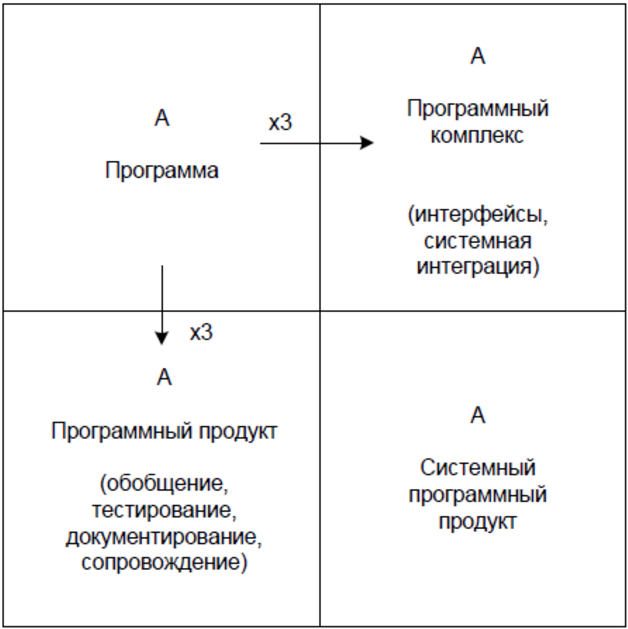
\includegraphics[width=0.5\textwidth]{brooksSquare.png}
	\end{center}
	\caption{Программа и системный программный продукт}
	\label{figure:brooksSquare}
\end{figure}

Проблема в том, что <<Программы>> в этом смысле никому не нужны. Умение создавать такого рода программы необходимо для программиста, но это далеко не всё, что от квалифицированного программиста требуется. Люди готовы платить деньги не за код, который работает у разработчика, а за код, который работает у них. Они хотят доверять программе в том плане, что программа не падает на каждый чих и, скорее всего, не испортит их данные. Они хотят понимать программу --- знать, как ей пользоваться, как её устанавливать и настраивать. Они хотят, чтобы программа работала с адекватной скоростью на их устройствах. Они хотят от программы чего-то нового, поэтому они хотят, чтобы разработчики не забрасывали программу, а продолжали поддерживать её, добавлять в неё новые возможности и править ошибки. Таким образом, ценность представляет не <<программа>>, а <<программный продукт>>, то есть та же программа, но оттестированная (покрытая модульными и интеграционными тестами), документированная (имеется пользовательская и техническая документация), с налаженным процессом сопровождения (налажен процесс исправления ошибок и выпуска новых версий), работающая на всех возможных входных данных и корректно обрабатывающая ошибочные ситуации. Брукс утверждает, что программный продукт примерно втрое более трудоёмок, чем программа, но на самом деле программный продукт может оказаться ещё дороже (одни только модульные тесты --- обычно количество строк кода в них сопоставимо с количеством строк кода продукта, а часто и превосходит).

Кроме того, очень многие практически полезные программы сейчас работают не сами по себе, а в составе программных комплексов, будь то отдельные сервисы в распределённых приложениях, утилиты в операционных системах, плагины в средах разработки и так далее. Современная корпоративная информационная система может состоять из десятков различных приложений, развёрнутых на десятках различных вычислительных узлов, и все они должны быть интегрированы в единую систему. Это влечёт дополнительные трудозатраты на описание интерфейсов и протоколов общения между приложениями, и на интеграционное тестирование, сложность которого вполне может расти экспоненциально в зависимости от количества интегрируемых приложений. Ну а действительно полезный результат работы --- это системный программный продукт, обладающий всеми описанными выше свойствами.

Таким образом, оказывается, что если требования к ПО невелики, его можно просто <<сесть и написать>>, но в современном мире требования к ПО велики, поэтому часто приходится ещё и думать о разных других характеристиках ПО, помимо функциональности. Собственно, архитектура в этом сильно помогает. Ещё насчёт <<сесть и написать>> есть проблема в том, что ПО может быть слишком большим для этого. Немного примеров приведено в таблице~\ref{table:loc}\footnote{по данным \url{http://www.informationisbeautiful.net/visualizations/million-lines-of-code/}}.

\begin{figure}
	\begin{tabu} {| X[0.5 l p] | X[1 l p] |}
		\tabucline-
		\everyrow{\tabucline-}
		Простая игра для iOS            & 10000 LOC \\
		Unix v1.0 (1971)                & 10000 LOC \\
		Quake 3 engine                  & 310000 LOC \\
		Windows 3.1 (1992)              & 2.5M LOC \\
		Linux kernel 2.6.0 (2003)       & 5.2M LOC \\
		MySQL                           & 12.5M LOC \\
		Microsoft Office (2001)         & 25M LOC \\
		Microsoft Office (2013)         & 45M LOC \\
		Microsoft Visual Studio 2012    & 50M LOC \\
		Windows Vista (2007)            & 50M LOC \\
		Mac OS X 10.4                   & 86M LOC \\
	\end{tabu}
	\caption{Количество строк кода в типичных программных проектах}
	\label{table:loc}
\end{figure}

Архитектура --- это как раз то, что в принципе позволяет создавать ПО размером больше 100000 строк кода. Без грамотной архитектуры большой проект рискует развалиться под собственной сложностью ещё в процессе разработки. 

Есть довольно большой сегмент рынка ПО, связанный с разработкой мобильных приложений или одностраничных веб-сайтов без сложной логики, такие приложения, как правило, небольшие, так что при их разработке можно обходиться без архитектурных навыков. Многие разработчики всю жизнь работают junior- или mid- developer-ами, получают задачи уже декомпозированными, и тоже обходятся без того, про что будет рассказываться в этом курсе. Все остальные вынуждены знать и уметь странные вещи типа паттернов, архитектурных стилей, UML и т.д., о чём и пойдёт речь далее.

\subsection{Что такое архитектура и зачем она нужна}

Общепринятого определения и даже понимания понятия <<Архитектура>> не существует, но на интуитивном уровне архитектура --- это набор важнейших решений об организации программной системы --- того, из каких компонентов она состоит, как эти компоненты взаимосвязаны друг с другом и с окружением, какие ограничения действуют на сами компоненты и взаимосвязи между ними, мотивация принятых решений. Стандарт ISO/IEC 42010 "Systems and software engineering --- Architecture description" определяет архитектуру как ``fundamental concepts or properties of a system in its environment embodied in its elements, relationships, and in the principles of its design and evolution''. Поскольку программые системы, как правило, очень сложны, архитектура системы разделяется на части, каждая из которых описывает систему с какой-то определённой точки зрения (по аналогии с архитектурой зданий, где есть поэтажный план здания, план электропроводки, план водопровода и т.д.), эти части называются архитектурными видами. При этом каждый вид может состоять из нескольких описаний (неформальных, полуформальных или на каком-нибудь формальном языке), и эти описания могут различаться по уровню детализации (опять-таки, проводя аналогию с архитектурой зданий, может быть модель здания целиком и детальный план каждого помещения). В отличие от архитектуры здания, архитектура программной системы меняется и эволюционирует вместе с самой системой --- ошибочные представления об архитектуре как деятельности, предшествующей программированию, я надеюсь, будут развеяны по ходу курса. Интересно то, что архитектура у системы есть всегда, даже если о ней никто не думал и никак её не описывал, просто она может оказаться не очень хорошей.

Для чего тратить усилия на явное описание архитектуры системы?
\begin{itemize}
	\item С создания первого варианта архитектуры начинается реализация системы, это та деятельность, которая даёт понять, что и примерно как нужно писать. Продуманная архитектура может \textbf{в разы} сократить затраты на кодирование.
	\item Архитектура --- это инструмент управления проектом. Даже оценить проект (а следовательно, принять решение, браться за него или нет) невозможно без декомпозиции задачи на подзадачи и выделения основных компонентов, крупнозернистая декомпозиция может определить состав команды и даже структуру организации, разрабатывающей систему. И по ходу выполнения проекта надо иметь чёткое представление о компонентах системы и связях между ними, чтобы понять, на каком этапе разработки мы сейчас находимся.
	\item Архитектура --- это средство обеспечения переиспользования, как третьесторонних компонентов, так и переиспользования внутри системы (или группы систем). Именно архитектура позволяет выделить возможные кандидаты на переиспользование, определить требования к третьесторонним компонентам, определить критерии выбора, выделить и инкапсулировать функциональность своих компонентов, чтобы сделать их переиспользуемыми.
	\item И главное, явное описание архитектуры системы позволяет делать выводы о некоторых её качествах ещё до того, как написана первая строчка кода. Несколько разных вариантов архитектуры может быть разработано и проанализировано, среди них может быть выбран вариант, наиболее подходящий для текущей ситуации и только после этого реализован. Формальные средства описания архитектуры позволяют иногда получать не только качественные, но и количественные характеристики системы, например, оценивать ожидаемую производительность или требуемую память. К сожалению, такие средства не очень распространены в промышленности, так что и в этом курсе мы их почти не коснёмся.
\end{itemize}

Интересно, что заказчику архитектура системы совершенно не интересна, они ожидают, что система будет делать то, что им нужно, причём хорошо и быстро. Как она устроена внутри, им особо не интересно. Как писал Алан Купер\footnote{А. Купер, Р.М. Рейманн, Д. Кронин, Алан Купер об интерфейсе. Основы проектирования взаимодействия, Символ-Плюс, 2009г, 688 С.}, если бы в магазинах продавали дырки в стене, никто не покупал бы дрели.

\subsection{Профессия <<Архитектор>>}

В крупных проектах архитектор --- это, как правило, специально выделенный человек или даже группа людей, в задачи которых входит разработка и описание архитектуры системы, доведение её до всех заинтересованных лиц, контроль реализации архитектуры и поддержание её в актуальном состоянии по ходу разработки и сопровождения проекта. Есть профессиональный стандарт <<Архитектор программного обеспечения>>, диплом <<Математическое обеспечение и администрирование информационных систем>> позволяет вести профессиональную деятельность и по этой профессии (почему, собственно, курс по архитектуре есть в программе подготовки). Стандарт определяет цель деятельности архитектора так:

{\ttfamily
Создание и сопровождение архитектуры программных средств, заключающейся 
	\begin{itemize}
		\item в синтезе и документировании решений о структуре;
		\item компонентном устройстве;
		\item основных показателях назначения; 
		\item порядке и способах реализации программных средств в рамках системной архитектуры; 
		\item реализации требований к программным средствам; 
		\item контроле реализации и ревизии решений
	\end{itemize}
}

Вот некоторые трудовые функции архитектора согласно этому же стандарту:

{\ttfamily
	\begin{itemize}
		\item Создание вариантов архитектуры программного средства
		\begin{itemize}
			\item Определение перечня возможных типов для каждого компонента
			\item Определение перечня возможных архитектур развертывания каждого компонента
			\item Определение перечня возможных слоев программных компонентов
			\item Определение функциональных характеристик и возможностей, включая эксплуатационные, физические характеристики и условия окружающей среды, при которых будет применяться каждый компонент
			\item Определение перечня возможных протоколов взаимодействия компонентов
			\item Определение перечня возможных механизмов авторизации
			\item Определение перечня возможных механизмов аутентификации, поддержки сеанса
			\item Определение перечня возможных схем кеширования
			\item ...
		\end{itemize}
		\item Документирование архитектуры программных средств
		\begin{itemize}
			\item Разработка документации программных средств в своей части
			\item Поддержка изменений в документации
		\end{itemize}
		\item Реализация программных средств
		\begin{itemize}
			\item Анализ качества кода: анализ зависимостей; статический анализ кода
			\item Испытания создаваемого программного средства и его компонентов
			\item Технические и управленческие ревизии создаваемого программного средства
		\end{itemize}
		\item Оценка требований к программному средству
		\item Оценка и выбор варианта архитектуры программного средства
		\item Контроль реализации программного средства
		\item Контроль сопровождения программных средств
		\item Оценка возможности создания архитектурного проекта
		\item Утверждение и контроль методов и способов взаимодействия программного средства со своим окружением
		\item Модернизация программного средства и его окружения
	\end{itemize}
}

Как видим, архитектор, помимо собственно разработки архитектуры, выполняет также техническое руководство проектом, контролирует ход его реализации, оценивает качество результата на всём протяжении разработки и даже сопровождения. Таким образом, архитектор --- это ключевой технический специалист в команде. Кроме того, на архитектора же чаще всего возлагают обязанности по коммуникации между разработчиками и руководством, часто архитектор принимает участие в общении с заказчиком, поэтому для архитектора важны не только технические, но и социальные навыки. Хороший архитектор должен обладать большим кругозором и уметь быстро погружаться в предметную область, в которой разрабатывается проект --- в отличие от программиста, которому обычно достаточно разбираться в той технологии, которую он использует для реализации. Картинка, иллюстрирующая соотношение знаний архитектора и разработчика, приведена на рисунке~\ref{figure:architectVsDeveloper}.

\begin{figure}
	\begin{center}
		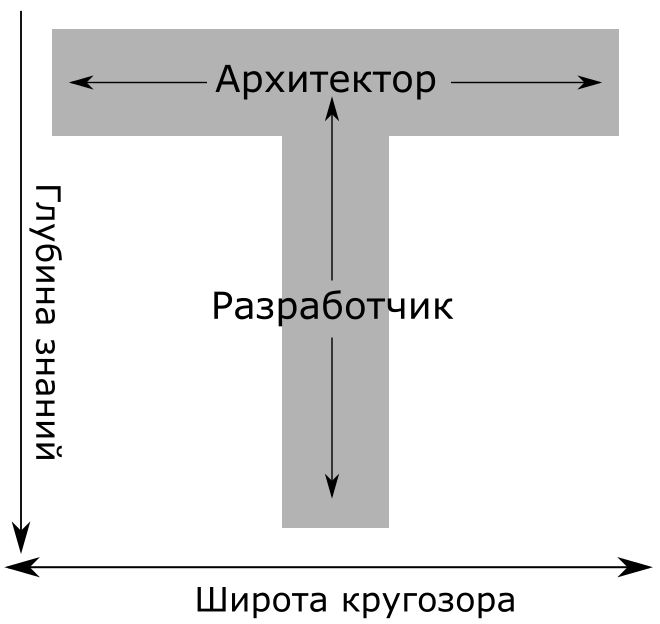
\includegraphics[width=0.4\textwidth]{architectVsDeveloper.png}
	\end{center}
	\caption{Знания архитектора и знания разработчика}
	\label{figure:architectVsDeveloper}
\end{figure}

Часть знаний и умений архитектора может прийти только с опытом, поэтому обычно будущему архитектору сначала приходится поработать на позиции разработчика. В небольших командах часто архитектор вынужден также исполнять функции разработчика, а часто и наоборот, разработчики вынуждены заниматься архитектурой помимо, собственно, кодирования. В общем-то, ничего страшного в этом нет, в отличие от строительства зданий в мире разработки ПО не удаётся достичь чёткого разделения труда как между архитектором и строителем (ведь программа по сути --- это проект, строит её компилятор), так что функции архитектора и разработчика перекрываются. Более того, если архитектор сидит <<в башне из слоновой кости>> и только говорит разработчикам, что делать, он быстро теряет связь с кодом и утрачивает понимание реализации. Это приводит к тому, что его архитектурные решения игнорируются разработчиками или, если архитектор настаивает, приводят к ухудшению качества системы. Поэтому хороший архитектор должен быть прежде всего опытным программистом и писать код вместе с командой (может быть, уделяя больше внимания интерфейсам компонентов, протоколам связи и интеграционным тестам, но всё-таки код). 

Но при этом архитектор не должен заниматься микроменеджментом и пытаться навязывать программистам своё видение реализации. Если задача декомпозирована до уровня конкретных методов классов, программистам будет неинтересно работать в таком проекте и они уйдут. Архитектору следует доверять программистам и оставлять реализационные аспекты им. По моему мнению, граница между ответственностью архитектора и ответственностью программиста проходит где-то на уровне паттернов проектирования из известной книжки Э. Гаммы\footnote{Must read: Гамма Э. и др. Приемы объектно-ориентированного проектирования. -- Издательский дом "Питер", 2016, 366С.}. С паттернами любой программист должен быть в состоянии разобраться самостоятельно, поэтому какие паттерны лучше использовать для реализации компонента --- уже скорее дело программиста, а вот что должен делать компонент и как он должен быть связан с остальными --- дело архитектора. Но паттерны проектирования в этом курсе всё равно будут, потому что это важная штука.

\section{Пример: ПО для осциллографа}

Посмотрим на примере, какое влияние архитектура оказывает на приложение и что примерно ожидается от архитектора. Рассмотрим некоторую компанию, которая занимается проектированием осциллографов --- да-да, устройств для записи параметров электрического сигнала\footnote{Пример и всё изложение в этом разделе позаимствованы из статьи Garlan D., Shaw M. An introduction to software architecture //Advances in software engineering and knowledge engineering. -- 1993. -- Т. 1. -- №. 3.4.}. Если раньше осциллографы были аналоговыми и никакого софта к ним было вообще не нужно, то сейчас осциллограф умеет считывать кучу параметров, оцифровывать их, сохранять во внутреннем хранилище, выполнять разные фильтрации и преобразования (например, преобразование Фурье), отображать результаты на экране (с тач-скрином, меню и встроенной справкой) и выдавать в сеть, где этими результатами могут пользоваться как обычные компьютеры, так и другие устройства. Эта наша компания выпускает сразу несколько разных моделей осциллографов, да ещё и предоставляет услугу настройки своей продукции под конкретные нужды конкретного клиента. Последнее раньше было просто (просто меняем прошивку осциллографа на слегка подправленную), но с ростом функциональности приборов стало сложно и дорого. Поэтому понадобилась Архитектура.

В первой версии архитектуры авторы пошли по пути создания объектно-ориентированной модели предметной области (как мы увидим далее, это наиболее распространённый и считающийся идеологически правильным сейчас подход, но авторы об этом не знали, 1993 год же). Были выделены основные сущности, определены связи между ними, нарисованы диаграммы в духе диаграммы из рисунка~\ref{figure:oscilloscopeObjects}\footnote{Оригинальная иллюстрация из всё той же статьи An introduction to software architecture}.

\begin{figure}
	\begin{center}
		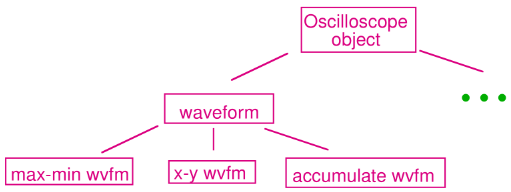
\includegraphics[width=0.6\textwidth]{oscilloscopeObjects.png}
	\end{center}
	\caption{Объектно-ориентированная модель осциллографа}
	\label{figure:oscilloscopeObjects}
\end{figure}

Это не дало желаемого результата, потому что хоть все сущности и были аккуратно выделены, их оказалось слишком много, а  разбить сущности на модули, компоненты или слои, объектная модель не помогала. Кроме того, было неочевидно, как разбить функциональность по объектам (например, измерения должны моделироваться как часть объектов, представляющих данные, которые измеряются, или как отдельные объекты). Сейчас все эти проблемы объектной модели более-менее известно, как решать, но тогда авторы решили отказаться от такого подхода и попробовать что-то ещё. Впрочем, результаты не пропали даром, объектная модель всё равно пригодилась, и главное, улучшила понимание предметной области архитекторами.

Следующая итерация была уровневой архитектурой: система разделялась на слои, самый нижний отвечал за взаимодействие непосредственно с оборудованием, на нём строился слой оцифровки и слой цифровой обработки, на нём слой визуализации, на нём --- слой пользовательского интерфейса, и, как это принято в уровневых архитектурах, каждый слой мог общаться только со слоем непосредственно выше или ниже его самого. Получилось что-то наподобие рисунка~\ref{figure:oscilloscopeLayers}\footnote{Тоже иллюстрация из статьи}.

\begin{figure}
	\begin{center}
		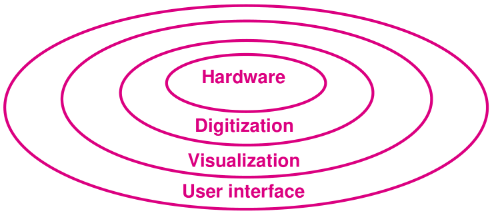
\includegraphics[width=0.6\textwidth]{oscilloscopeLayers.png}
	\end{center}
	\caption{Уровневая модель осциллографа}
	\label{figure:oscilloscopeLayers}
\end{figure}

Такая модель (заметим, что внутри слоёв вполне могли использоваться объекты из предыдущей) была проста для понимания и хорошо структурировала всю систему. Однако она тоже оказалась не очень, потому что на самом деле все слои должны были знать про все остальные слои, например, пользовательский интерфейс должен был позволять настраивать параметры оцифровки и различных преобразований, в виде графиков могли отображаться не только результаты хитрых вычислений, но и <<сырой>> сигнал. Все преимущества слоистого подхода при таком положении вещей терялись, поэтому авторы продолжали работать над архитектурой получше.

Следующая модель --- <<каналы и фильтры>> --- модель, рассматривающая функциональность осциллографа как набор последовательных преобразований над данными. Концепция такой архитектуры изображена на рисунке~\ref{figure:oscilloscopeFilters}\footnote{Опять-таки, иллюстрация из статьи}.

\begin{figure}
	\begin{center}
		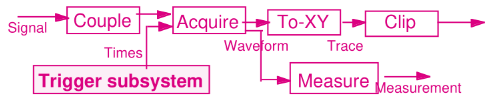
\includegraphics[width=0.6\textwidth]{oscilloscopeFilters.png}
	\end{center}
	\caption{Модель осциллографа, основанная на потоке данных}
	\label{figure:oscilloscopeFilters}
\end{figure}

Теперь ничто не мешает пользовательскому интерфейсу показывать <<сырой>> сигнал, к тому же такая точка зрения на систему близка к точке зрения пользователей осциллографа --- инженеров. Однако пользовательские настройки всё ещё не очень хорошо ложились в эту модель, потому что если пользовательский интерфейс мог быть только в конце <<трубопровода>>, то получалось ещё хуже, чем в слоистой модели, когда пользователь на самом деле не мог ничего менять, а если интерфейс мог быть повсюду, получалась каша хуже той, что была в чисто объектной модели.

Поэтому архитектура был слегка модифицирована, фильтрам добавили возможность принимать два разных типа данных --- данные, с которыми фильтры, собственно, работали и передавали дальше, и управляющие сигналы, см. рисунок~\ref{figure:oscilloscopeModifiedFilters}.

\begin{figure}
	\begin{center}
		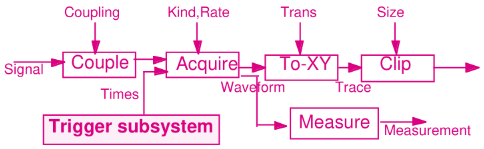
\includegraphics[width=0.6\textwidth]{oscilloscopeModifiedFilters.png}
	\end{center}
	\caption{Модель осциллографа, основанная на потоке данных с управляющими входами}
	\label{figure:oscilloscopeModifiedFilters}
\end{figure}

Теперь всё было хорошо, настройки моделировались как управляющие входы, отображаться могло всё, что угодно, и главное, система была легко расширяема и конфигурируема --- достаточно было описать новый тип фильтра, описать его связи с существующими фильтрами, и так получить новую функциональность для осциллографа. Так что на этой (точнее, на немного улучшенной, но по сути этой) архитектуре авторы и решили остановиться.

\subsection{Выводы}

Из этого примера видно, что мы можем делать какие-то утверждения о свойствах разрабатываемой системы, базируясь исключительно на её структурных свойствах, не написав ни строчки кода и даже не выбрав язык реализации. Причём, структура системы оказывает очень сильное влияние на весь ход проекта: в первом варианте, с чистой объектно-ориентированной моделью система оказывалась несопровождаемой и нерасширяемой в долгосрочной перспективе, во втором варианте, со слоями, и в третьем, с каналами и фильтрами система не могла красиво с точки зрения реализации удовлетворить функциональным требованиям. Естественно, можно было во время реализации <<затолкать>> в архитектуру нужную функциональность, например, <<пробросить>> данные и параметры конфигурации через несколько слоёв, сделав функции, просто делегирующие вызов на слой ниже, но это опять-таки удорожило бы разработку и сопровождение.

Ещё из примера видно, что все наши рассуждения носят весьма оценочный и субъективный характер. Это тоже весьма типично для архитектуры, есть формальные методы, позволяющие получить количественные результаты, но всё равно, большая часть принимаемых решений не может быть объективно оценена. Архитектура --- это во многом гуманитарная область, архитектура системы создаётся для людей и предназначена прежде всего для упрощения понимания людьми структуры системы. Архитектура должна объяснять и упрощать, а эти вещи сложно оценить и сложно сравнивать. Поэтому часто оказывается, что всей команде приходится полагаться на интуицию и чувство вкуса архитектора. Из этого же следует, что не бывает <<правильной>> или <<неправильной>> архитектуры. Какой бы ужас вы ни породили, скорее всего, его удастся ценой некоторых усилий реализовать так, чтобы он таки заработал. Тем не менее, бывают архитектуры явно удачные и явно не удовлетворяющие требованиям, однако отличить одну от другой заранее очень сложно (особенно если требования заранее неизвестны, как чаще всего и бывает). Страшного в этом ничего нет, потому что архитектура меняется во время жизни приложения, так что ошибки можно исправить. Но это может стоить довольно дорого, например, архитектурный рефакторинг проекта QReal:Robots\footnote{Образовательная среда программирования роботов, \url{https://github.com/qreal/qreal/tree/master/plugins/robots}} потребовал примерно человеко-года усилий. Причём надо помнить, что во время архитектурного рефакторинга добавлять полезную функциональность и вообще развивать продукт не получится.

Третье наблюдение состоит в том, что архитектурные подходы, которые мы применяли, не специфичны для осциллографов. Уровневое разбиение, которое тут нам не подошло, вполне успешно применяется в сетевых протоколах (например, модель OSI --- типичная уровневая архитектура), объектно-ориентированная модель предметной области --- основа структуры типичных информационных систем и заодно основа их схемы баз данных. Собственно, обобщения таких подходов называются архитектурными стилями, это что-то вроде архитектур архитектуры --- архитектурный стиль определяет основные структурные элементы конкретной архитектуры и ограничения на них. Архитектура у каждой системы своя, а вот известных архитектурных стилей не так уж много, поэтому любой адекватный архитектор должен их знать. Поэтому у нас в курсе будет отдельная пара с обзором стилей и несколько пар с их подробным обсуждением.

Четвёртый вывод из примера состоит в том, что систему можно рассматривать с разных точек зрения. Первый вариант архитектуры, с объектами, концентрировался на статической структуре системы и описывал сущности, из которых система состоит. Третий вариант, с фильтрами, концентрировался на потоках данных, которые существуют в системе, их преобразованиях и взаимосвязях. Также можно заметить и разные уровни детализации --- разбиение системы на слои явно более <<крупнозернисто>>, чем разбиение на конкретные классы, кроме того, дальше не детализируется --- нет никакого смысла разбивать слои на подслои и т.д. В какой-то момент каждый слой должен быть представлен моделью с классами, так что если бы слоистая архитектура нам подошла, она состояла бы минимум из двух разных видов описаний. Такие описания называют \emph{архитектурными видами} (architectural view), а совокупность видов, рассматривающая систему единообразно --- \emph{архитектурной точкой зрения} (architectural viewpoint). Например, диаграмма классов и диаграмма <<сущность-связь>> --- это два разных вида, относящиеся к одной точке зрения.

\section{Архитектурное описание, архитектурные виды}

По поводу архитектурных видов подробно написано в стандартах IEEE 1016-2009 <<Software Design Descriptions>> и ISO/IEC/IEEE 42010:2011 <<Architecture description>>. IEEE 1016 выделяет аж 12 точек зрения на систему:
\begin{itemize}
	\item Контекст  --- описывает, что система должна делать, фиксирует окружение системы. Состоит из сервисов и акторов, которые могут быть связаны информационными потоками. Система представляет собой <<чёрный ящик>>. Корень иерархии уточняющих дизайн системы видов, стартовая точка при проектировании системы. Обычно описывается с помощью диаграмм активностей UML, IDEF0 (SADT).
	\item Композиция --- описывает крупные части системы и их предназначение. Предназначен для локализации и распределения функциональности системы по её структурным элементам, impact analysis-а, облегчения переиспользования (в том числе, покупки компонентов), оценки, планирования, управления проектом, определения необходимой инструментальной поддержки (репозитории, трекер и т.д.). Обычно описывается с помощью диаграмм компонентов UML, IDEF0, Structure Chart.
	\item Логическая структура --- структура системы в терминах классов, интерфейсов и отношений между ними. Типичные языки --- диаграммы классов UML, диаграммы объектов UML.
	\item Зависимости ---  определяет связи по данным между элементами: разделяемая между элементами информация, порядок выполнения и т.д. Необходим для анализа изменений, идентификации узких мест производительности, планирования, интеграционного тестирования. Типичные языки --- диаграммы компонентов UML, диаграммы пакетов UML.
	\item Информационная структура --- определяет персистентные данные в системе (информация, которую требуется хранить, схема БД, доступ к данным). Типичные языки --- диаграммы классов UML, IDEF1x, ER, ORM
	\item Использование шаблонов --- документирование использования локальных паттернов проектирования. Типичные языки --- диаграммы классов UML, диаграммы пакетов UML, диаграммы коллабораций UML.
	\item Интерфейсы --- специфицирует информацию о внешних и внутренних интерфейсах, не прописанную явно в требованиях. Пользовательский интерфейс рассматривается отдельным видом в рамках этой точки зрения. Типичные языки --- IDL, диаграммы компонентов UML, макеты пользовательского интерфейса, неформальные описания сценариев использования.
	\item Структура системы --- рекурсивное описание внутренней структуры компонентов системы. Типичные языки --- диаграммы композитных структур UML, диаграммы классов UML, диаграммы пакетов UML.
	\item Взаимодействия --- описывает взаимодействие между сущностями: почему, когда, как и на каком уровне выполняется взаимодействие. Типичные языки --- диаграммы композитных структур UML, диаграммы взаимодействия UML, диаграммы последовательностей UML.
	\item Динамика состояний --- описание состояний и правил переходов между состояниями в реактивных системах. Типичные языки --- диаграммы конечных автоматов UML, диаграммы Харела, сети Петри.
	\item Алгоритмы --- описывает в деталях поведение каждой сущности, логику работы методов. Типичные языки --- диаграммы активностей UML, псевдокод, настоящие языки программирования.
	\item Ресурсы --- описывает использование внешних ресурсов (как правило, аппаратных или третьесторонних сервисов). Типичные языки --- диаграммы развёртывания UML, диаграммы классов UML, OCL.
\end{itemize}

Хорошая новость в том, что все эти архитектурные виды необязательны, стандарт требует только общие сведения о системе (назначение, границы системы, контекст, в котором система существует) и те виды, которые архитектор считает важными.

Можно обратить внимание, сколько раз в стандарте упоминаются UML и другие языки моделирования (что интересно, сам стандарт использует диаграммы классов UML для описания своих основных концепций и терминов). Модели вообще очень важны для архитектуры системы, потому что ПО само по себе очень сложно, а модели по определению упрощают сложное, оставляя существенное. К несчастью, модели ПО, в отличие от математических и физических моделей, принципиально не могут быть простыми, потому что сложность ПО --- это то самое, с чем работает архитектура, от сложности нельзя абстрагироваться и объявить её несущественной. Но для этого, собственно, и придуманы виды --- каждый вид рассматривает свой какой-то аспект системы, сложность каждого вида ограничена, хотя сложность всей системы может быть сколь угодно большой.

С языками визуального моделирования, в особенности с UML, мы ещё познакомимся подробно в этом курсе. UML --- это общепринятый промышленный стандарт, так что уметь читать UML-диаграммы надо всем, даже тем, кто хочет всю жизнь проработать младшим разработчиком, а умение рисовать UML-диаграммы --- обязательный навык для любого архитектора, даже если в каком-то конкретном проекте или организации ими  не пользуются.

\section{Роль архитектуры в жизненном цикле ПО}

Есть распространённое заблуждение, что работа архитектора напрямую связана с фазой проектирования жизненного цикла ПО --- архитектор получает проанализированные требования от аналитиков, рисует диаграммы, пишет design document, отдаёт всё, что получилось, программистам на реализацию и идёт заниматься следующим проектом. В некоторых компаниях, между прочим, так и делают, практика <<кочующих архитекторов>> довольно эффективна по стоимости, поскольку можно держать одну опытную архитектурную команду, обслуживающую сразу много проектов. Тем не менее, современная точка зрения на архитектуру больше склоняется к тому, что архитектура это непрерывная активность, находящаяся в центре процесса разработки, см., например, рисунок~\ref{figure:architectureLifeCycle} из книги Z. Quin, ``Software Architecture''\footnote{Z. Quin, J. Xing, X.Zheng, ``Software Architecture'',  Zhejiang University Press, 2008, 337pp}. Создание, поддержка и эволюция архитектуры --- это такие же деятельности, необходимые на всех этапах жизненного цикла, как контроль версий или управление проектом, архитектура при этом ещё и направляет остальные деятельности.

\begin{figure}
	\begin{center}
		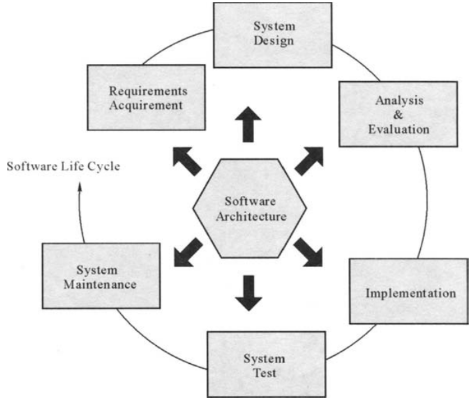
\includegraphics[width=0.6\textwidth]{architectureLifeCycle.png}
	\end{center}
	\caption{Место архитектуры в жизненном цикле ПО}
	\label{figure:architectureLifeCycle}
\end{figure}

Много кто пишет, что собирать требования надо безотносительно конкретной реализации, чтобы требования отражали потребности пользователя, а не то, что мы ему (иногда подсознательно) навязали исходя из своих возможностей по реализации. Тем не менее, сбор и анализ требований --- это уже архитектурная активность, в этот момент рисуются первые модели системы, пишутся первые документы, которые лягут в основу будущей архитектуры, а затем и реализации. Например, диаграмма случаев использования UML, пример которой представлен на рисунке~\ref{figure:useCaseDiagram}, она показывает роли пользователей системы и доступную им функциональность. Нередко в сборе требований и общении с заказчиком участвует архитектор.

\begin{figure}
	\begin{center}
		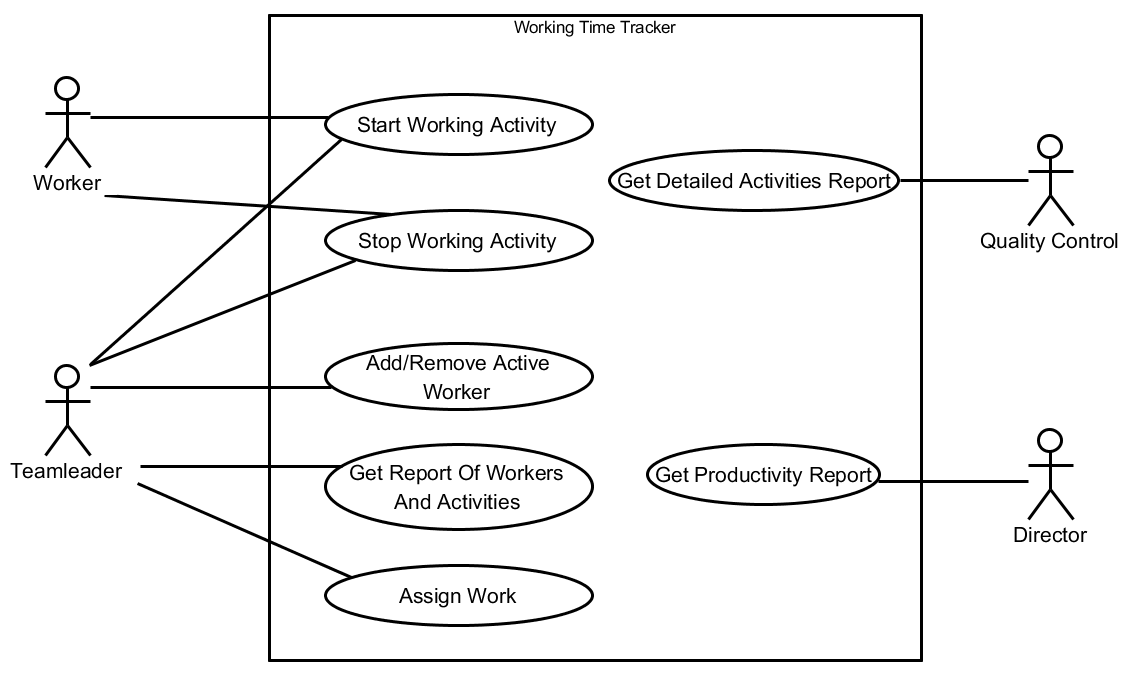
\includegraphics[width=0.6\textwidth]{useCaseDiagram.png}
	\end{center}
	\caption{Диаграмма случаев использования UML}
	\label{figure:useCaseDiagram}
\end{figure}

Требования вообще чрезвычайно важны для архитектуры, поскольку это исходные данные для проектирования. Напомним, что требования бывают таких типов.
\begin{itemize}
	\item Функциональные --- то, \emph{что} система должна делать.
	\item Нефункциональные --- то, \emph{как} система должна это делать.
	\begin{itemize}
		\item Требования на эффективность по времени работы и по используемым ресурсам.
		\item Требования на масштабируемость --- насколько адекватно система справляется с ростом нагрузки.
		\item Требования на удобство использования --- насколько легко учиться пользоваться системой и насколько удобно собственно пользоваться ею.
		\item Требования на надёжность.
		\begin{itemize}
			\item Время наработки на отказ --- сколько времени в среднем система работает без отказов.
			\item Время восстановления после сбоя --- за сколько времени систему можно восстановить, если она всё-таки отказала. Заметим, что время наработки на отказ и время восстановления после сбоя --- это разные вещи, имеющие разное значение в разных ситуациях. Например, для межпланетного зонда  время восстановления после сбоя может быть вообще не интересно, если мы неправильно сориентировали антенну, то всё, он навсегда потерян в глубинах космоса, тогда как время наработки на отказ критично --- если зонду лететь 20 лет, но в среднем раз в два года бортовое ПО падает с критической ошибкой, запускать такой зонд бессмысленно. Для сотового телефона наоборот, один пропущенный из-за сбоя вызов не страшен, если можно быстро перезвонить.
			\item Корректность поведения при сбое (failsafe) --- есть системы, в которых даже критическая ошибка должна приводить к корректному завершению работы (классический пример с ядерным реактором и с банковской системой).
		\end{itemize}
		\item Требования на безопасность.
		\item Требования на сопровождаемость и расширяемость.
		\item ...
	\end{itemize}
	\item Ограничения
	\begin{itemize}
		\item Технические --- например, если вы программируете под iPhone, то ограничены в выборе инструментария.
		\item Бизнес-ограничения --- например, система должна быть сделана за месяц, иначе на уже назначенной пресс-конференции будет нечего показать.
	\end{itemize}
\end{itemize}

Наибольшее влияние на архитектуру оказывают, как ни странно, нефункциональные требования. Дело в том, что написать работающую программу, в общем-то, не сложно, и это можно сделать миллионом различных способов. Сложно сделать так, чтобы она была ещё и быстрой, сопровождаемой, надёжной и т.д. Поэтому и архитектурный стиль выбирается исходя из приоритетов нефункциональных требований, и архитектура проектируется в большой степени с их учётом.

На стадии проектирования архитектурные вопросы естественным образом оказываются в центре внимания. Обратите внимание, что сейчас мало где используется водопадная модель разработки, поэтому стадию проектирования проекты чаще всего проходят несколько раз (например, в начале каждой итерации в agile-методологиях). На фазе проектирования выполняется декомпозиция задачи, определяются границы компонентов, определяются интерфейсы и протоколы общения. На стадии проектирования же решаются вопросы, общие для всей системы: стратегия обработки ошибок, стратегия логирования, стратегия выкатывания обновлений и т.д. На стадии проектирования же создаётся большая часть архитектурной документации. Для этого опять-таки оказываются полезны визуальные языки, например, диаграммы компонентов UML, которые показывают <<вид с высоты птичьего полёта>> на систему. Например, высокоуровневая архитектура прошивки робота представлена в виде диаграммы компонентов на рисунке~\ref{figure:trikRuntimeComponents}.

\begin{figure}
	\begin{center}
		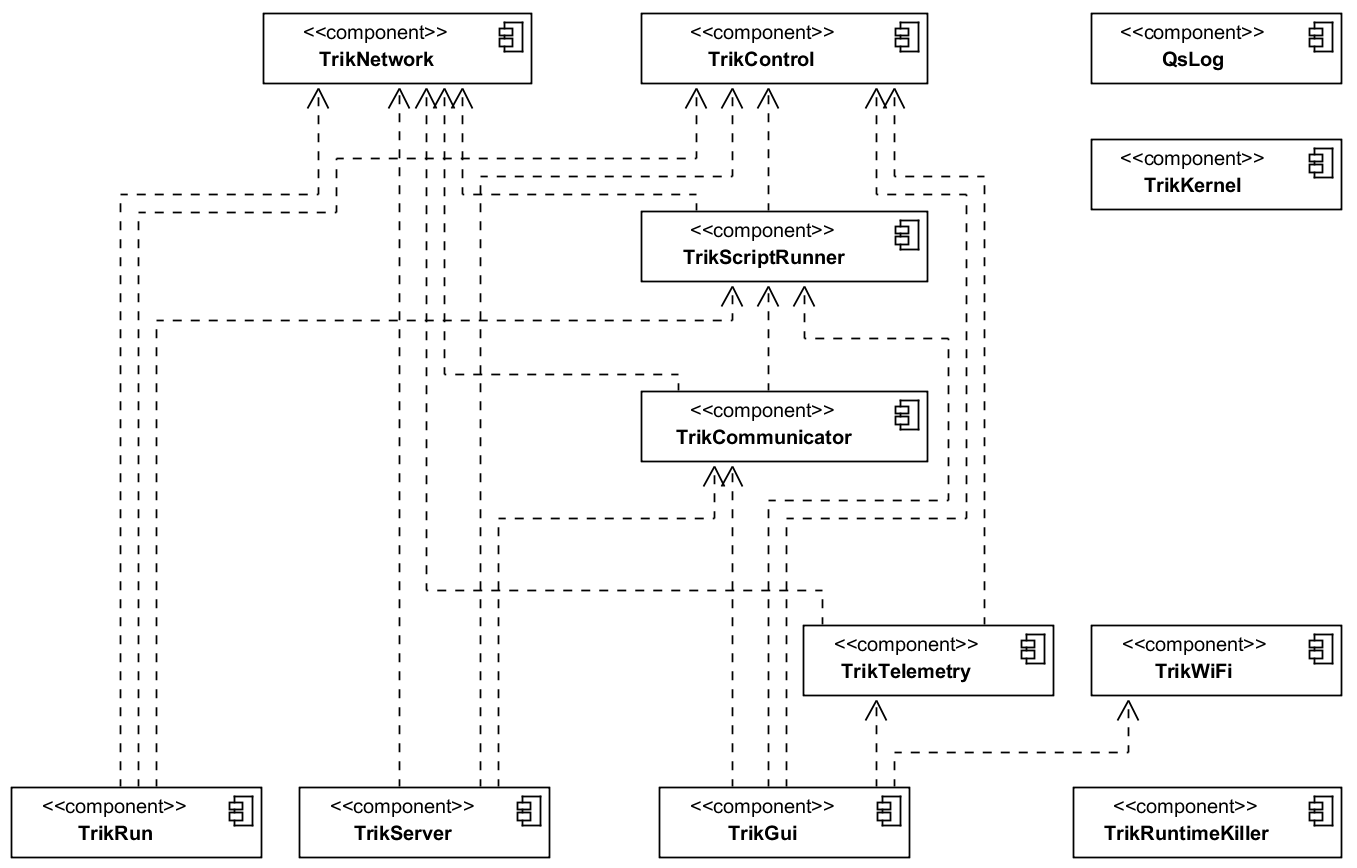
\includegraphics[width=\textwidth]{trikRuntimeComponents.png}
	\end{center}
	\caption{Диаграмма компонентов UML}
	\label{figure:trikRuntimeComponents}
\end{figure}

На фазах реализации, тестирования и поддержки за архитектурой необходимо следить, причём, как правило, делать это приходится вручную --- архитектурные ограничения редко удаётся формализовать так, чтобы они могли проверяться инструментами. Архитектура может быть подвержена двум видам проблем. Первая из них --- это \emph{architectural drift} --- появление в <<фактической>> архитектуре системы (которая, кстати, называется <<\emph{descriptive architecture}>> --- <<описывающая архитектура>>) важных архитектурных решений, которых не было в разработанной архитектуре (которая, в свою очередь, называется <<\emph{prescriptive architecture}>> --- <<предписывающая архитектура>>). Такие решения вполне могут ничего не ломать и быть вполне адекватными, но, как правило, оказываются незадокументированными, никто не задумывался об их <<глобальных>> последствиях, они применяются только к части системы, не становясь общим принципом, что, разумеется вносит свою долю хаоса. Вторая проблема --- это \emph{architectural erosion} --- нарушение в фактической архитектуре системы принципов, заложенных в её предписывающей архитектуре. Поскольку архитектурные ограничения сложно проверять автоматически, архитектурная эрозия возникает на практике очень часто в процессе багфиксов, рефакторингов, добавления новой функциональности, и, опять-таки, даже если напрямую ничего не ломает, вносит хаос в систему (в гораздо большей степени, чем drift) и постепенно превращает систему в <<большой ком грязи>>, где всё связано со всем и никто не знает, как оно работает. Архитектурная эрозия чем-то похожа на законы термодинамики и энтропию. Бороться с эрозией, так же, как и с энтропией, в общем-то, бесполезно --- надо помнить, что каждый рефакторинг, каждый багфигс, каждая написанная новая строка кода имеет свою цену в виде потениальной архитектурной эрозии и сползания проекта в хаос. Хорошая и чётко описанная архитектура, постоянное внимание архитектора и архитектурные рефакторинги могут сильно замедлить этот процесс.

Тем не менее, в жизненном цикле системы может наступить момент, когда внесение изменений становится слишком дорогим из-за сильной эрозии архитектуры. В это время может потребоваться \emph{восстановление архитектуры} по имеющемуся коду, рефакторинг этой архитектуры и далее глобальный рефакторинг кода для того, чтобы привести его в соответствие новой архитектуре. В особо запущенных случях может потребоваться применять методы реинжиниринга (например, если архитектурная документация вообще утеряна). В любом случае, процесс это сложныи и долгий, причём, пока выполняется такая работа, никакое развитие системы невозможно.

\end{document}
